\documentclass[spanish]{beamer}
\usepackage[ansinew]{inputenc} % Acepta caracteres en castellano
\usepackage[spanish]{babel}    % silabea palabras castellanas
\usepackage{amsmath}
\usepackage{mathtools,cancel} % cancela con una flecha \cancelto{0}{XXXX}
\renewcommand{\CancelColor}{\color{red}} %change cancel color to red
\usepackage{amsfonts}
\usepackage{amssymb}
\usepackage{dsfont}
\usepackage{graphicx}
\usepackage{geometry}
\usetheme{Madrid}
\usecolortheme{beaver}
\usepackage{textpos}
% Logo  en el comienzo 
\addtobeamertemplate{frametitle}{}{%
\begin{textblock*}{100mm}(.85\textwidth,-1cm)
{\includegraphics[height=0.4in, keepaspectratio=true]{/Users/luisnunez/Dropbox/MisDocumentos/UIS/UISImagenInstitucional/UISLOGO.png}}
\end{textblock*}}

\begin{document}

\title{\textbf{Peque�as oscilaciones} }
\author[L.A. N��ez]{\textbf{Luis A. N��ez}}  
\institute[UIS]{\textit{Escuela de F�sica, Facultad de Ciencias, } \\
\textit{Universidad Industrial de Santander, Santander, Colombia } \\
{\includegraphics[height=0.4in, keepaspectratio=true]{/Users/luisnunez/Dropbox/MisDocumentos/UIS/UISImagenInstitucional/UISLOGO.png}}
}
\date{\today}
\maketitle


\begin{frame}
\frametitle{Agenda}
  \tableofcontents
\end{frame}


%%%%% Diapo 1
\section{Peque�as oscilaciones 1D}
\frame{
  \frametitle{Peque�as oscilaciones 1D 1/2}
   \begin{itemize}  
  	\item<1-> Como vimos en la clase de estabiliad dado un $\mathcal{L}=\frac{1}{2} c\dot{q}^2-V_{\mathrm{ef}}(q)$
	\item<2-> La ecuaci�n de movimiento es $c \ddot{q}=f_{\mathrm{ef}}(q) \equiv -\frac{\partial V_{\mathrm{ef}}}{\partial q}$
	\item<3-> Que tendr� un m�nimo en $q_0$, cuando  $f_{\mathrm{ef}}\left(q_0\right)=\left.0 \Rightarrow \frac{\partial V_{\mathrm{ef}}}{\partial q}\right|_{q_0}=0$
	\item<4-> Ser� estable si $\left.\frac{\partial V_{\mathrm{ef}}^2}{\partial q^2}\right|_{q_0}>0$
	\item<5-> Igual que en el caso anterior perturbamos alrededor del m�nimo
	\begin{figure}[t]
		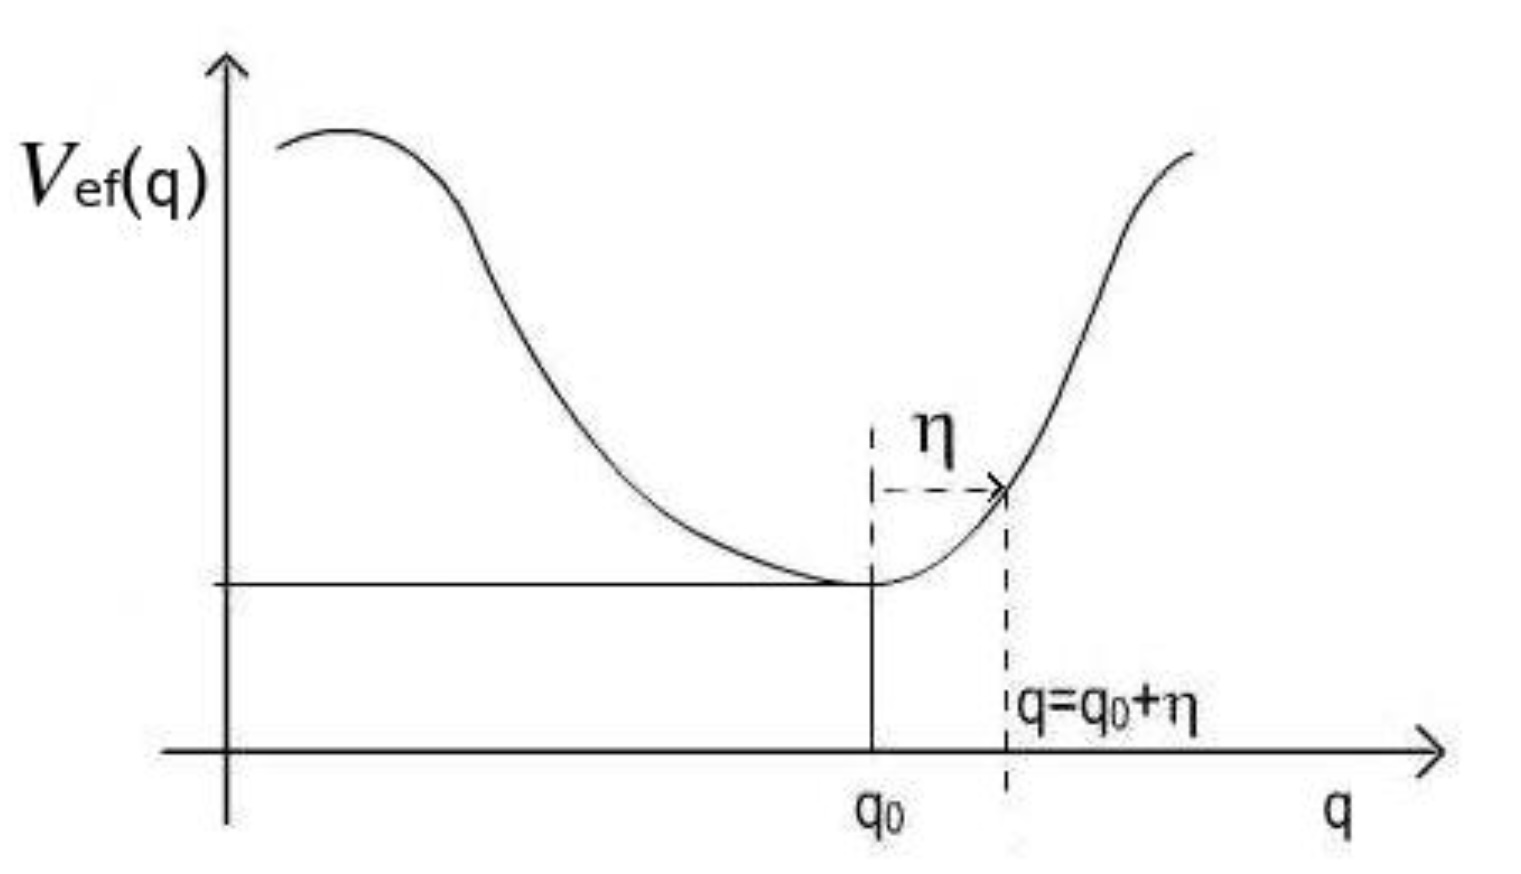
\includegraphics[width=1.8in]{Figuras/MinimoOscila.jpg}
   	\end{figure}
	\item<6-> Desarrollamos por Taylor, $V_{\text {ef }}(q)$ alrededor de $q=q_0$, y tenemos  $V_{\mathrm{ef}}(q)=V_{\mathrm{ef}}\left(q_0+\eta\right)=V\left(q_0\right)+ \cancelto{0}{\left.\frac{\partial V_{\mathrm{ef}}}{\partial q}\right|_{q_0}} \eta+\left.\frac{1}{2} \frac{\partial^2 V_{\mathrm{ef}}}{\partial q^2}\right|_{q_0} \eta^2+\cdots,$
    \end{itemize}
}
%%%%% Diapo 2
%\section{Peque�as oscilaciones 1D}
\frame{
  \frametitle{Peque�as oscilaciones 1D  2/2}
  \begin{itemize}  
  	\item<1-> Despreciando t�rminos en potencias de $\eta$ de orden superior al cuadr�tico, tenemos $V_{\mathrm{ef}}(q)=V_{\mathrm{ef}}\left(q_0+\eta\right) \approx \frac{1}{2} K\left(q-q_0\right)^2=\frac{1}{2} K \eta^2$
	\item<2-> La ecuaci�n de movimiento ser� $c \ddot{\eta} =-\frac{\partial V_{\text {ef }}}{\partial q}=-K\left(q-q_0\right) \equiv -K \eta$
	\item<3-> Entonces, $\ddot{\eta}+\omega^2 \eta=0$, donde $\omega^2 \equiv \frac{K}{c}=\left.\frac{1}{c} \frac{\partial^2 V_{\mathrm{ef}}}{\partial q^2}\right|_{q_0}$ es la frecuencia angular de las peque�as oscilaciones alrededor de $q_0$.
	\item<4-> Que tendr� como soluci�n \\ $\eta(t)=c_1 \cos \omega t+c_2 \operatorname{sen} \omega t=A \cos (\omega t+\varphi) \equiv \operatorname{Re}\left[A e^{i(\omega t+\varphi)}\right]=\operatorname{Re}\left(a e^{i \omega t}\right)$ donde $a=A e^{i \varphi}$ es la amplitud compleja

   \end{itemize}
}
%%%%% Diapo 2
\section{Oscilaciones con varios grados de libertad}
\frame{
  \frametitle{Oscilaciones con varios grados de libertad}
  \begin{itemize}  
  	\item<1-> Dado un sistema con $s$ grados de libertad $\left\{q_i: i=1, \ldots, s\right\}$ con energ�a potencial  $V\left(q_1, \ldots, q_s\right)$.
	\item<2-> La configuraci�n de equilibrio del sistema en $\left\{q_{0 i}: i=1, \ldots, s\right\}$, con $\left.\frac{\partial V}{\partial q_i}\right|_{q_{0 i}}=0, \quad i=1,2, \ldots, s$
	\begin{figure}[t]
		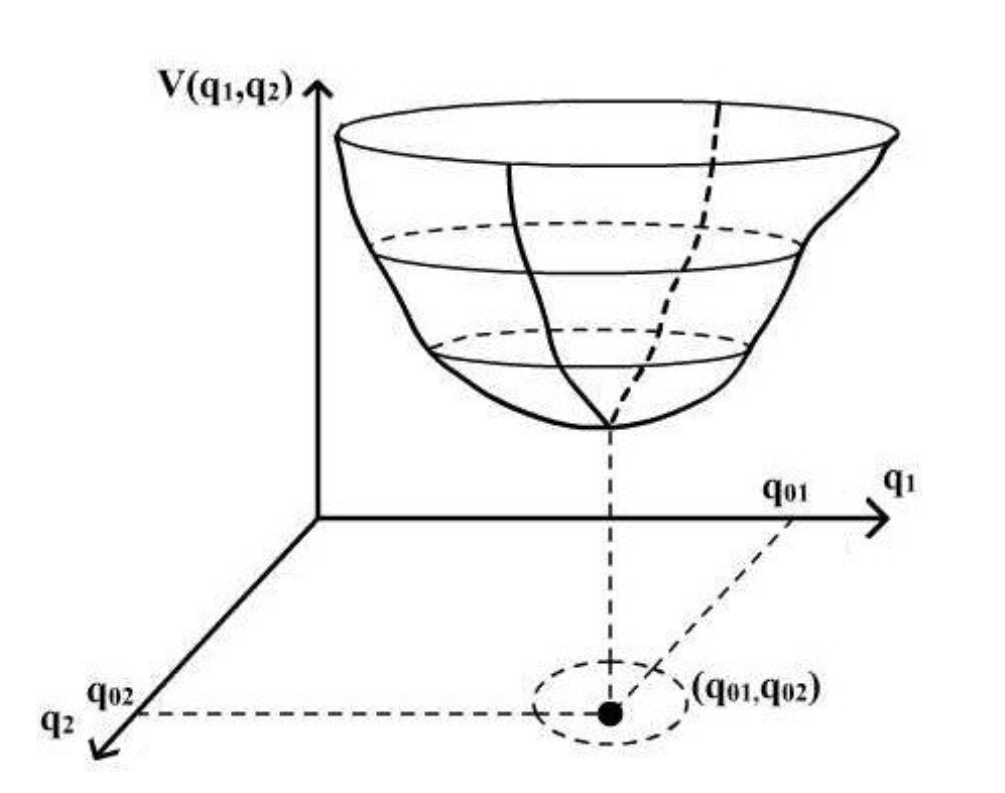
\includegraphics[width=1.8in]{Figuras/OscilaVariosGrados.png}
   	\end{figure}
	\item<3-> Perturbando las $q_i$, tendremos $q_i=q_{0 i}+\eta_i,$  con $\eta_i \rightarrow 0 \quad \left(\frac{\eta_i}{q_{0 i}} \ll 1\right)$
	\item<4-> El valor del potencial $V\left(q_1, \ldots, q_s\right)$ cerca de la configuraci�n de equilibrio se obtiene de la expansi�n de Taylor en varias variables de $V\left(q_1, \ldots, q_s\right)$ alrededor de $\left\{q_{0 i}\right\}$, con $q_i=q_{0 i}+\eta_i$,
   \end{itemize}
}
%%%%% Diapo 2
%\section{Secci�n}
\frame{
  \frametitle{Oscilaciones con varios grados de libertad 2/2}
  \begin{itemize}  
  	\item<1-> Esto es 
	$V\left(q_1, \ldots, q_s\right)=V\left(q_{01}, \ldots, q_{0 s}\right)+ \cancelto{0}{\sum_i\left(\frac{\partial V}{\partial q_i}\right)_{\left\{q_{0 i}\right\}}} \eta_i +\frac{1}{2} \sum_i \sum_j\left(\frac{\partial^2 V}{\partial q_i \partial q_j}\right)_{\left\{q_{0 i}\right\}} \eta_i \eta_j+\cdots$ 
	\item<2-> Los $V\left(q_{01}, \ldots, q_{0 s}\right)$ es un valor constante y las derivadas parciales est�n evaluadas en $\left\{q_{0 i}\right\}=\left(q_{01}, \ldots, q_{0 s}\right)$.
	\item<3-> En la configuraci�n de equilibrio $q_i=q_{0 i}+\eta_i$, el potencial se puede expresar como $V\left(q_1, \ldots, q_s\right)=V\left(\eta_1, \ldots, \eta_s\right)=\frac{1}{2} \sum_{i, j} V_{i j} \eta_i \eta_j$
	\item<4-> donde los coeficientes $V_{i j} \equiv\left(\frac{\partial^2 V}{\partial q_i \partial q_j}\right)_{\left\{q_{0 i}\right\}}$ son sim�tricos, $V_{i j}=V_{j i}$

   \end{itemize}
}
%%%%% Diapo 2
\section{Secci�n}
\frame{
  \frametitle{T�tulo transparencia}
  \begin{itemize}  
  	\item<1-> 
   \end{itemize}
}
%%%%% Diapo 2
\section{Secci�n}
\frame{
  \frametitle{T�tulo transparencia}
  \begin{itemize}  
  	\item<1-> 
   \end{itemize}
}
%%%%% Diapo 2
\section{Secci�n}
\frame{
  \frametitle{T�tulo transparencia}
  \begin{itemize}  
  	\item<1-> 
   \end{itemize}
}  
\end{document}
